\documentclass[12pt,halfline,a4paper,nonumbib]{ouparticle}

%\usepackage[authoryear]{natbib}

\usepackage[backend=biber,
            style=authoryear,
            %citestyle=authoryear,
            maxcitenames=1,
            sorting=nyt]{biblatex}
\addbibresource{references.bib}

%% My definitions
\usepackage{xcolor}
\newcommand{\todo}{\textcolor{red}}
\newcommand{\disp}{\displaystyle}

\usepackage{algorithm}
\usepackage{algorithmicx}
\usepackage{algpseudocode}

\usepackage{setspace}
\doublespacing

\usepackage{lineno}
\linenumbers

%\usepackage{subcaption}

\begin{document}

\title{Validation of stock assessment models using prediction skill: Is it me or my model talking? 
%For as the eyes of bats are to the blaze of day, so is the reason in our soul to the things which are by nature most evident of all.
}

\author{%
  \name{Laurence T. Kell}
  \address{ Centre for Environmental Policy, Imperial College London, Weeks Building, 16-18 Princes Gardens, London\\ SW7 1NE, UK}
  \email{laurie@seaplusplus.co.uk}
  \and
  \name{Rishi Sharma}
  \address{Food and Agricultural Organization, Fishery and Aquaculture Policy and Resources Division, Rome, Lazio,\\
    00153, Italy}
  \email{rishi.sharma@fao.org}
  \and
  \name{Toshihide Kitakado}
  \address{Department of Marine Biosciences, Tokyo University of Marine Science and Technology, 4-5-7 Konan, Minato, Tokyo \\108-8477, Japan}
  \email{e-mail address}
  \and
  \name{Henning Winker}
  \address{Joint Research Centre (JRC), European Commission, TP 051, Via Enrico Fermi 2749, 21027 Ispra, VA, \\Italy.}
  \email{e-mail address}
  \and
  \name{Iago Mosqueira}
  \address{Wageningen Marine Research, Haringkade 1, 1976CP IJmuiden, \\The Netherlands.}
  \email{iago.mosqueira@wur.nl}
  \and
  \name{Massimiliano Cardinale}
  \address{Swedish University of Agricultural Sciences, Department of Aquatic Resources, Institute of Marine Research, Lysekil,\\ Sweden}
  \email{massimiliano.cardinale@slu.se}
  \and
  \name{Dan Fu}
  \address{ Indian Ocean Tuna Commission, Le Chantier Mall, Po Box 1011, Victoria – Seychelles’}
}

\abstract{
  The adoption of the Precautionary Approach requires a consideration of uncertainty, which is commonly addressed by the use of alternative stock assessment model structures and data sets. Evaluating models using goodness-of-fit diagnostics based on model residuals and likelihoods, however, can be difficult in such cases, while retrospective analysis based on model outputs can not be used to validate a model as this requires a reference set of observations. Moreover, although, these diagnostics tell us how well we describe the past, they tell us little about how well we  predict the future under alternative management actions. We, therefore, develop a procedure based on hindcasting for model validation based on prediction skill. To demonstrate the approach we compare alternative model structures based on integrated statistical and Bayesian state-space biomass dynamic models using Indian Ocean yellowfin tuna.  Validation is not a binary process (i.e. pass or fail) but a continuum, we therefore discuss how prediction skill can be used to identify alternative hypotheses, weight individual models within an ensemble or agree a reference set of operating models when conducting Management Strategy Evaluation.}

\date{\today}

\keywords{cross-validation, diagnostics, hindcasting, prediction skill, retrospective analysis, stock assessment, validation.}

\maketitle

\section{Introduction}

There are various definitions of stock assessment \parencite[e.g.][]{hilborn2003state,cadrin2014stock}, our preference is for ``The description of the characteristics of a 'stock' so that its biological reaction to being exploited can be rationally predicted and the predictions tested" (Sidney Holt pers comm.). The reasoning for this is  because it explicitly recognises that the main aim of a stock assessment is to provide the basis for the long-term sustainable management of fisheries. The adoption of the Precautionary Approach to fisheries management \parencite[PA,][]{garcia1996precautionary} requires a formal consideration of uncertainty, which is often addressed by the use of different modelling frameworks, assumptions and data sets. Stock assessment, therefore, requires making and validating probabilistic estimates of stock status and forecasts of the consequences of different management actions. 

Diagnostic tests are essential for determining the robustness of model estimates used to provide management advice \parencite{carvalho2020cookbook}. It can be challenging, however, to use traditional diagnostics based on model residuals and likelihoods as for example AIC (Akaike’s Information Criteria  \parencite[AIC,][]{akaike1998information}) to compare models. Indices of abundance are an important contributor to the overall likelihood when fitting stock assessment models to data \parencite{whitten2013accounting}, and the sum of squared errors (SSE) between observed and predicted indices in log-space is the measure of fitness. The use of SSE is problematic because complex models tend to have many parameters to allow flexibility when fitting, which may result in a low SSE due to overfitting. Therefore, information criteria, such as AIC, have been developed to aid in model selection. AIC, however, needs to be performed on models with the same likelihood function and data, which is often not the case in stock assessment, where different hypotheses may be modeled with completely different model structures requiring different data sets. In addition, AIC is only a relative measure of the appropriateness of models and so additional diagnostic tests are required. This is of particular importance for stock assessment models where only a single historical data set exists, and the system can not be observed. 

A standard diagnostic method in stock assessment to check the stability of model estimates is retrospective analysis \parencite{hurtado2014looking}. The procedure involves sequentially removing all data from the most recent period, refitting the model, and comparing terminal year model estimates of spawning stock biomass (SSB) and fishing mortality ($F$) to the full model. The diagnostic is widely used around the world, and in Europe it is often the "key diagnostic" for accepting or rejecting a model \parencite{GFCM2020, ICES2019}. Retrospective analysis has been extended to include stock forecasts, where the terminal year estimates are projected using assumptions about future catches, recruitment, biological parameters and the vulnerability of the stock to fishing \parencite[e.g.][]{brooks2016retrospective}. Stability and a reduction in variance, however, can be achieved at the expense of accuracy and bias, for example by shrinking terminal estimates towards recent historical values. It is not possible, however, to validate a model if bias is unknown and the quantity used for validation is not observable \parencite{hodges1992you}. 

An alternative to SSE, AIC and retrospective analysis is to use prediction skill \parencite{glickman2000glossary}. Prediction skill is a measure of the accuracy of an estimate compared to observed values that are not known by the model. In supervised machine learning cross-validation is widely used to prevent overfitting since although learning the parameters of a prediction function and testing it on the same data may achieve a perfect fit, it might fail to predict anything useful on unseen data. Common practice when performing machine learning therefore is to hold back part of the available data and compare model estimates to observed values \parencite{jin2008current, weigel2008can, balmaseda1995decadal}. 

  
Model validation is essential in many fields, e.g. climate and energy modelling \parencite{kell2019optimising}, since it increases confidence in the outputs of a model and leads to an increase in trust amongst the public, stake and asset-holders and policymakers \parencite[][]{saltelli2020five}. A variant of cross-validation is the hindcast or backtest, where like retrospective analysis, recent data are held back and the model refitted. Known values (observations) or well estimated historical values are then compared to model estimates (predictions). The former approach is also referred to as model-free and the latter as model-based validation \parencite{kell2016xval}. Observations can be peeled back from the terminal year and then predictions are made by 1, 2, ... n steps ahead, they may be removed by series to evaluate data conflicts, fleets, time blocks to overcome serial correlations, or individually to estimate bias using the jackknife. No stock forecast or projection needs to be performed and so there is no need to make assumptions about future parameters as these are estimated within the model.  
%Therefore, we conducted a hindcast by removing observations, generated pseudo observations, and then compared these to the observations omitted. The procedure is non-parametric and is applicable to any automated model building technique. It can provide important diagnostic information about influential cases in the data set and the stability of the model \parencite{michaelsen1987cross}. It can therefore be used to validate models, identify model misspecification, data conflicts, and where models need to be modified or extended.

Current literature \parencite[e.g.][]{deroba2014simulation}, however, primarily focuses on the past, and how well models fit these data. Historical performance, however, is no indicator of how well a model may perform in the future, which is a key objective of fisheries management. Thus, the goal of the paper is validate models using prediction skill, defined as a measure of the accuracy of a predicted value compared to an actual observed value that is not known by the model. We are not proposing validation as the only diagnostic tool to be used in stock assessment, but as a key tool for use in the assessment toolbox \parencite{carvalho2020cookbook}. As a worked example, we compare three model families used for the assessment of Indian Ocean yellowfin tuna stock, namely a full integrated statistical model \parencite[SS,][]{methot2013stock}, an age-structured production model \parencite[ASPM,][]{maunder2015contemporary}, and a Bayesian state-space biomass dynamic model \parencite[JABBA,][]{winker2018jabba}.


\section{Material and Methods}

We conduct model-based and model-free hindcasting to estimate prediction skill using as a worked example yellowfin tuna (\textit{Thunnus albacares}), based on the most recent assessment conducted by the Indian Ocean Tuna Commission \parencite{IOTWPTT21}. 

After a model structure is agreed, it is crucial to validate the model to assesses whether it is plausible that a system identical to the model generated the data \parencite{thygesen2017validation}. The ambition of validation is not to prove that a model is correct, but to check that the model can not be falsified with the available data. This is a different question from asking is the model fit for a given purpose, which depends on the intended use of the model. For example, to evaluate whether an assessment model is robust  despite being misspecified, Management Strategy Evaluation \parencite[MSE,][]{punt2007developing} can be conducted. See \parencite{sharma2020trfmo} for a review of current practice in the tuna Regional Fisheries Management Organisations (tRFMOs). Validation is not a binary process, i.e. identifying whether a model is valid or invalid, as there is a continuum between these two extremes. A primary objective of validation is therefore not to try and select a "best assessment" but to identify if models are overfitted and how they can be extended or modified to better describe the dynamics.

Model validation serves a complementary purpose to model selection and hypothesis testing. Model selection searches for the most suitable model within a specified family, hypothesis testing examines how to reduce the model structure, while model validation examines if the model should be modified or extended. For models to be valid, they must satisfy four prerequisites \parencite{hodges1992you}. Namely, the situation modelled must: i) be observable and measurable; ii) be possible to collect sufficient data informative about it; iii) Exhibit constancy of structure in time; and iv) exhibit constancy across variations in conditions not specified in the model

The first two prerequisites should be straight forward; however, many stock assessments, particularly for highly migratory stocks like yellowfin fished in areas beyond national jurisdiction, rely on fishery-dependent data rather than direct scientific observations. The use of fishery-dependent data is a concern since \parencite{harley2001catch} it has been found strong evidence that commercial catch per unit effort (CPUE) is likely to remain high while abundance declines.  Prerequisite (iii) ensures that the model has prediction skill for the same conditions under which the validation tests were conducted, and prerequisite (iv) ensures that the model will still be valid under conditions that differ from those in the validation tests.

\subsection{Materials}

Yellowfin tuna supports one of the largest tuna fisheries in the Indian Ocean, with catches currently exceeding 400,000t annually. The stock is harvested by a variety of gears, from small-scale artisanal fisheries to large gillnetters, and industrial longliners and purse seiners \parencite{fiorellato2019tt}.
There are regional differences in the distribution of the stock and fisheries (figure \ref{fig:map}), and the  western tropical region (region 1) is considered the core area of the stock's distribution.

The majority of data available for assessing the stock is fishery dependent. These include time series of total catch, seasonal catch per unit effort (CPUE) based on the long-line fisheries \parencite{hoyle2020scaling}, samples of length compositions, tagging recaptures, and environmental data. CPUE are the primary source of information on abundance and are based on a composite long-line index,  spatially stratified by region, from the main distant water fleets. %\parencite{hoyle2018yft}. 

Indices in each region are standardised using generalised linear models that accounted for differences in targeting practices and catchability amongst fleets, based on gear configurations and species composition \parencite{hoyle2020scaling}. The reason for this is because tuna long-line fishing strategies have changed over time. %\parencite{hampton2005}. 
In the assessment, the CPUE indices across regions were linked by a common catchability coefficient, thus improving the ability of the model to estimate the distribution of biomass by region. %\parencite{langley2015yft, fu2018yft}.

The length composition are considered sufficient to provide reasonable estimates of fishery selectivity and recruitment trends but not trends in stock abundance. Regional environmental indices (current and sea temperature) allow seasonal and temporal variations to be incorporated in the estimation of fish movement. Tag release and recovery data collected from the main phase of the Indian Ocean large-scale tuna tagging programme %[Hallier 2008] 
inform estimates of mortality, abundance, and movement. 


\subsection{Assessment Models}

Model development has focused on spatial structure to account for differences in regional exploitation patterns. Non-stationarity in selectivity and catchability, and seasonal movements have been found to resolve data conflicts  \parencite{urtizberea2018yft}. Although a full integrated statistical model is used to develop the base case, other families of models are also used.  These include  an age-structured production model \parencite[ASPM,][]{maunder2015contemporary} and a Bayesian state-space biomass dynamic model \parencite[JABBA,][]{winker2018jabba}. 

Stock Synthesis \parencite[SS,][]{methot2013stock} is used to conduct the main assessment, and implements an age and spatially structured model that reflects the complex population and fishery dynamics of the stock. The most recent assessment established a base-case as a reference model for diagnostics along with scenarios to capture a range of uncertainties \parencite{fu2018yft}. The assessment indicates that the stock has declined substantially since 2012, and spawning stock biomass in 2017 is now estimated to be close to the historical lowest level. The stock is estimated to be overfished, and the IOTC has implemented a rebuilding plan to reduce overall fishing pressure.  

%There has been a recent trend in stock assessment toward the use of integrated analysis that combines several sources of data into a single model by a joint likelihood for the observed data \parencite[e.g.][]{doubleday1976least,fournier1982general,maunder2013review}. data sets include records of catches and landings, indices of abundance based on catch per unit (CPUE) or from research surveys, and length and age compositions based on samples. An example of an integrated assessment method is SS that can be configured in multiple ways, allowing for a range of scenarios to be developed to reflect uncertainty.

SS provides a flexible framework for conducting stock assessment and \cite{maunder2015contemporary} proposed a deterministic implementation of an age-structured production model (ASPM) in SS as a diagnostic of processes that control the shape of the production function \parencite{carvalho2017can}. Selectivity in ASPM is parameterised based on the selectivity estimated by a "full" SS model. The model is then fitted to the abundance indices, without the size composition data contributing to the likelihood function. Recruitment deviations can either be estimated (as in our example) or set to zero. This enables an evaluation of whether the observed catches alone can explain trends in the index of abundance. If the ASPM is able to fit the indices of abundance well then a production function is likely to exist (i.e. the dynamics are driven by density-dependent processes), and the indices provide information about absolute abundance. If the fit is poor, then the catch data alone cannot explain the trends in the indices. This can have several causes, namely (i) stock dynamics are recruitment-driven, (ii) the stock has not yet declined to the point at which catch is a major factor influencing abundance; (iii) the indices of relative abundance are not proportional to abundance;  (iv) the model is incorrectly specified; or (v) the data are incorrect. While a production function was evident in the fit, the overall fit to the indices of abundance in 3 of the 4 areas was poor, and hence we used recruitment deviates to help capture the trends in abundance by area \cite[see][]{minte2017get}.

An alternative to an integrated assessment is to use a biomass dynamic model, based on an explicit production function, this requires the estimation and fixing of fewer parameters. We used JABBA that presents a unifying, flexible framework for biomass dynamic modelling, runs quickly, and generates reproducible stock status estimates \parencite{winker2018jabba}. A Pella Tomlinson production function \parencite{pella1969generalized} was assumed as this allows the shape of the production function to be varied, and alternative assumptions about productivity, stock status and reference points to be evaluated. To make analyses comparable priors for the JABBA production function parameters were based on the SS base case. 

\subsection{Assessment Hypotheses}

The base case is spatially disaggregated into two tropical regions (R1 and R4) and two austral subtropical regions (R2 and R3). The tropics encompass the main year-round fisheries, while the long-line fisheries occur more seasonally in the austral regions \parencite{langley2015yft}, reciprocal movement is assumed to occur between adjacent regions. The base case assumes a quarterly time step to approximate the continuous recruitment and rapid growth seen in the stock. The population comprised 28 quarterly age-classes with an assumed unexploited equilibrium initial state in each region. Twenty-five fisheries are defined based on fishing gear, region, time period, fishing mode and vessel type. Fisheries were modelled allowing flexibility in selectivity (e.g. cubic spline or double normal), whereas long-line selectivity was constrained to be fully selective for the older ages. 

Recruitment occurs in the two equatorial regions with temporal deviates in the regional distribution and is assumed to follow a Beverton and Holt stock-recruitment relationship %(with a steepness of 0.8 and recruitment standard deviation of 0.6).  
Growth is parameterised using age-specific deviates on the $k$ growth parameter to mimic the non-von Bertalanffy growth of juvenile and the near linear growth of adults. Natural mortality is variable with age, with the relative trend in age-specific natural mortality based on the values applied in the Pacific Ocean \parencite{maunder2012review}. 

%[Maunder, M.N., Aires-da-Silva, A. 2012. A review and evaluation of natural mortality for the assessment and management of yellowfin tuna in the eastern Pacific Ocean. External review of IATTC yellowfin tuna assessment. La Jolla, California. 15-19 October 2012. Document YFT-01-07.]


\subsection{Hindcast}

In a retrospective analysis all observations for a year are sequentially removed from the terminal year backwards (i.e. peeled), the model is then refitted to the truncated series and model estimates compared to see if there are any systematic patterns. 

Validation, however, requires that the system be observable and measurable and so model free quantities should be used, unless model estimates are known to be very close to their true values. In stock assessment, however, bias is difficult to quantify. For example a reduction in mean squared error (a measure of variance) can be achieved by shrinkage at the expense of prediction skill. The absence of retrospective patterns in model based quantities, therefore, while reassuring is not sufficient for validation. Validation should therefore be conducted using prediction skill based on observations. We therefore used the models to generate pseudo data based on CPUE and compare these to observations. 
%When conducting the hindcast it is assumed that modelled variables are observable, processes exhibit constancy of structure in time, including those not specified in the model, and that collection of accurate and sufficient data is possible \parencite{hodges1992you}.

Hindcasting like retrospective analysis involves fitting a model using a tail-cutting procedure, where data are deleted sequentially. This may be done for individual data series or combinations of different series, for example fleets where both CPUE and length data are removed. This allows data conflicts to be explored. Theoretically, the projection period is to the end of the historical time period, however, in practice, a step size of one or several years ahead (the horizon $h$) is chosen. This reflects the time horizon required for robust management advice; considering non-small process stochasticity in fishery population dynamics and non-ignorable extents of observation uncertainty. 
%We  define `retro-period' and `hc-period' as `the period of shrunken data set for retrospective model fitting' and `future time period (i.e. horizons) with a certain projection step (say $S \geq 1$) for hindcasting after retro-period''. 
Assessment cycles are typically for three years in most tuna Regional Fisheries Management Organisations and so an horizon of three years was used.

In the procedure used in this study only CPUE observations were removed, catch and length composition remained in the model. Time series of pseudo data were generated from estimates of vulnerable biomass and catchability ($q$). Prediction residuals ($e$) were then computed as the difference between the predictions and the observations. %Hindcasting was not conducted with the length composition data, as it has been demonstrated that following the length data is often misleading if it conflicts with the abundance data \parencite{francis2011data}. In addition, in the case of the Indian Ocean yellowfin assessment length had been down weighted significantly so that they did not conflict with the indices of abundance \parencite{fu2018yft}. Keeping the catch data meant that it was not necessary to run a projection as an additional step.

%Finally, \cite{minte2017get} demonstrate for BET in the eastern Pacific following the length data can often lead to model misspecification and discuss the trade off of larger uncertainty due to estimating deviates based on indices rather than being more precise but off scale when using the length data, particularly if other parameters such as the life history of the species is misspecified.

\subsubsection{Relative Error}
 
In a retrospective analysis Mohn's $\rho$ \parencite{mohn1999retrospective}, is commonly used as a measure of relative error. We use a variant, as we scaled by the mean so the metric is not affected by the length of the peel or the number of step aheads.

\begin{equation}
\label{eqn:mohn}
\rho_{M} = \disp \frac{1}{n} \sum_{t=T-n}^{T-1} \frac{\hat{y}_{(1:t),t}-\hat{y}_{(1:T),t}}{\hat{y}_{(1:T),t}} 
\end{equation}

\noindent
where , $n$ is the number of time steps that the peel is performed for, $t$ is the time for which the missing value is being estimated, $T$ is the terminal year in the time series, and $\hat{y}$ denotes a model based quantity. The value with suffix $\hat{y}_{(1:T)|t}$ means a value estimated at time $t$ from the full series running from time 1 to $T$, and $\hat{y}_{(1:t),t}$ is the value estimated using the data window from 1 to $t (\leq T)$. 

$\rho_M$ is an average of the relative differences at the final time of each window, and is a measure of relative retrospective `bias' (scale-free) in a statistical sense. The metric tends to be applied not on the log but the original scale because both the directions of positive and negative bias are regarded as being equivalent. $\rho$ can be estimated for different horizons 
\begin{equation}
\label{eqn:mohn2}
\rho_{M} = \disp \frac{1}{n-h+1} \sum_{t=T-n}^{T-h} \frac{\hat{y}_{(1:t)|t+h}-\hat{y}_{(1:T)|t+h}}{\hat{y}_{(1:T)|t+h}} 
\end{equation}

For reference values which are low relative to the alternative there is no upper limit, while in the reverse case the error cannot exceed 1.0. Therefore, in practice its usual to use a lower bound of -0.15 and an upper bound of 0.20 to identify acceptable performance \parencite{hurtado2014looking}. For values near or equal to 0, e.g. stocks where exploitation or stock size is low, small absolute differences can result in large relative differences.  This may result in assessments being rejected when they are needed the most, e.g. during the development of recovery plans, when both stock biomass and fishing mortality may be low. 

\subsubsection{Prediction Skill}

Prediction skill based on a forecast compares an observation at time $t$ ($y_t$) to an estimate of that observation made $h$ time steps previously ($\hat{y}_{t|t-h}$). To do this we use the mean absolute scaled error (MASE), as it is a robust and easy to interpret statistic \parencite{hyndman2006another}. The MASE compares prediction error ($e_t$) for a prediction horizon of $h$ 

\begin{equation}
\label{eqn:err}
 e_t = y_t -\hat{y}_{t|t-h} 
\end{equation}

\noindent 
to a benchmark forecast corresponding to a na\"{i}ve forecast equal to the last observed value. 

\begin{equation} 
\hat{y}_{t|t-h}=y_{t-h}
\end{equation}

\noindent For a peel of $n$ and a horizon of $h$ years

\begin{equation}
\label{eqn:skill}
MASE=\frac{\frac{1}{n+1}\sum_{t=T-n}^{T} \left| y_t - \hat{y}_{t|t-h} \right|}{\frac{1}{n+1+h}\sum_{t=T-n-h}^{T} \left| y_{t} - {y}_{t-h}\ \right|}
%\frac{\frac{1}{n+1} \sum _{t=T-n}^{T}\left|y_t - \hat{y}_{t|t-h}\right|}{
%                  \frac{1}{n+1+h} 
%                  \sum_{t=T-n-h}^{T}\left|{y_{t} - {y}}_{t-h}}\right|} \\
\end{equation}

The MASE has the desirable properties of scale in-variance so can be used to compare forecasts across data sets with different scales, predictable behaviour, symmetry, interpretability and asymptotic normality. Unlike relative error MASE does not skew its distribution even when the observed values are close to zero, is easy to interpret as a score of 0.5 indicates that the model forecasts are twice as accurate as a na\''{i}ve baseline prediction. The Diebold-Mariano test \parencite{diebold1995comparing} for one-step forecasts can also be used to test the statistical significance of the difference between two sets of forecasts, i.e. by comparing the prrediction $y_t -\hat{y}_t$ to a random walk $y_t-y_{t-1}$. 

\section{Results}

The 1-step ahead (equivalent to a retrospective analysis) and the 3-step ahead predictions for model based quantities are presented in figure \ref{fig:retro} and summarised in table \ref{tab:retro-rho}. These show estimates of stock size - $SSB$ or biomass ($B$) - and exploitation level - fishing mortality ($F$) or harvest rate ($U$) - relative to their maximum sustainable yield ($MSY$) reference points.

No retrospective pattern is seen for ASPM, either for the traditional one (figure \ref{fig:retro}) or three-step (figure \ref{fig:retro3})  ahead forecasts. For SS a negative bias is seen in $SSB/SSB_{MSY}$ for 1-step ahead, while for the 3-step ahead forecast $SSB$ is overestimated in the recent period; little change is seen in the estimates of $F/F_{MSY}$. JABBA shows a slightly negative retrospective patterns for harvest rate, which increases for the forecast. In the case of JABBA although exploitation is less than the ${MSY}$ level stock biomass still declines below $B_{MSY}$, which implies that process error rather than the production function is driving the future dynamics. $\rho$ has to be in the range $[-0.15,0.2]$ for an assessment to be accepted, and all the assessments apart for the SS estimates of F pass the $\rho_{M_r}$ test. When the 3 year projection is considered, however, only ASPM shows acceptable performance. 

The results from the model-free hindcasts are shown in Figures~\ref{fig:hy} and \ref{fig:hy3} for the one and three year ahead predictions respectively. The background colour indicates whether MASE $\le 1$. Table \ref{tab:mase} summarises the MASE values. For SS and JABBA, prediction skill is poor for CPUE indices 2 and 4; the ASPM also performs poorly for Area 2. Prediction skill deteriorates for the three step ahead projection, particularly for the SS and JABBA; although for ASPM, CPUE indices for regions 1 and 3 still have good prediction skill. 

The model and prediction residuals for future periods from 1 to 5 steps ahead are summarised in Figure \ref{fig:residuals} pooling across all CPUE indices. SS becomes increasingly imprecise and biased as the prediction horizon is increased. Although JABBA is more precise, it is still biased.

\section{Discussion}

Of the three structurally different model families used to assess Indian Ocean yellowfin, it was found that the model with the best prediction skill was the ASPM. The poor performance of the base case assessment model that integrated all the available data is likely related to large sampling error in the length compositions, which therefore introduce noise rather than information about year-class strength. The Bayesian state-space biomass dynamic model, by contrast, produced reasonable performance metrics for the core fishing area (Region 1) and the south-western Indian Ocean (Region 3), but could not predict the diverging trends in CPUE for the Eastern Indian Ocean (Regions 3 and 4). It appears, therefore, that it is important for this stock to model both the age structure and spatial dynamics, while the quality of length samples needs to be improved. 

There are many aspects of resource dynamics and productivity about which there is little information in stock assessment data sets \parencite[e.g.][]{lee2011m,lee2012steepness, jiao2012modelling,simon2012effects,mangel2013perspective,pepin2015reconsidering,cury2014resolving}. Therefore hypotheses about different plausible states of nature are increasingly represented by alternative model structures, fixed parameters, and weighting of data components \parencite[][]{sharma2020trfmo}. Thus, as well as methods for identifying uncertainties and agreeing on scenarios \parencite{leach2014elicit}, there is a need for methods to weight, reject, and extend models to include alternative hypotheses, and to evaluate the value-of-information associated with different data sets. 

Model selection, however, based on methods like AIC are only suitable for comparing frameworks based on the same input data. There is also a danger, with diagnostics based on the inspection of residuals, of "hypothesis fishing" or "p-hacking" \parencite{wasserstein2016asa,head2015extent}, i.e. finding a pretext for excluding an index or adding extra parameters %\parencite[e.g.][]{schirripa2017hypothesis}
to improve the fit. While If multiple true hypotheses are tested, some of them will likely be rejected falsely. Thus, it is valuable to reserve part of the data for model-free validation, so that a pattern’s significance is not tested on the same data set that suggested the pattern \parencite{arlot2010survey}.


The accuracy and precision of predictions depend on the information in the data, and determines how far ahead we can predict and the potential uses of the model. If a model can not be validated there are still other uses, however, including the use of a model as part of a feedback management system and scenario modelling when conducting Management Strategy Evaluation (MSE). An example of a model that can not be validated is a catch only model where if catch observations are removed can not be run. It can be simulation tested however as part of an MP, since feedback means that there is no need for prediction skill.

\section{Conclusions}

The hindcast is an important tool to achieve the aims of this paper which was to support the definition of stock assessment "as the description of the characteristics of a ’stock’ so that its biological reaction to being exploited can be rationally predicted and the predictions tested." Since a model is to be used for forecasting, model predictions should be compared to observable and measurable properties of the system \parencite{ianelli2016multi}. 

The objective of validation is not to prove that a model is correct, but to check that the model can not be falsified with the available data. In other words if a model has poor prediction skill then you either need more informative data or to develop alternative models. This is a step forward from hypothesis testing and model selection which is a way of rejecting rather than extending models. 

Hindcasting enables objective comparison among models with different structures and data sets, which is challenging to do with conventional diagnostics based on likelihoods and model residuals. The hindcast procedure extends a commonly used diagnostic, retrospective analysis. Retrospective analysis assesses the temporal stability of advice to be evaluated using a reference series of model estimates based on the most recent assessment. It is not possible, however, to estimate bias using model-based and thus latent quantities. Instead, model estimates need to be compared to observations for objective model validation. We therefore calculated prediction skill using pseudo observations to identify overfitting and to explore how models can be improved based on alternative structural assumptions without the risk of ‘hypothesis fishing’. 

The approach can also be used with an ensemble of models to develop robust advice, either for providing estimates of current stock status or by conducting MSE. For example, backtesting is a form of hindcasting and is used for evaluating the relative performance of alternatives strategies by comparing these to historical results. It is used in financial risk modelling to assess the performance of a trading or investment strategy. This requires simulating past conditions which is simple with the hindcast. Conducting MSE as part of the backtest allows the impact of feedback on historical catches and stock status to be evaluated. The problem is that it is possible to find a strategy that would have worked well in the past, but will not work well in the future. Therefore, although a backtest MSE is useful, particularly as it allows stakeholders to see what the consequences would have been if a different strategy had been employed, it is not sufficient to ensure the robustness of a strategy to be applied in the future. Despite this limitation, backtesting provides insights that may not be available when models and strategies are tested on simulated data alone and can be performed before conducting MSE for future years.

Another promising field of applications is to use the hindcast procedure to weight multi-model ensembles using skill-based weighting. Here, a prediction skill score can be used to assign more weight on the better performing models as this has been found to improve forecasts \parencite[e.g.][]{casanova2009weighting}. This can be done to weight estimates of current status relative to reference points, or weight operating models. Testing the approach on an actual case study first was informative as it provides the insight necessary to set up a study on synthetic data.

As the stock assessment process become more complex, e.g. through the increased use of integrated models, ensembles of models, and MSE, there are concerns about a lack of transparency. This is because of the many internal, implicit and often poorly documented assumptions, and a lack of access as only a few highly skilled experts are able to run the models \parencite{hilborn2003state}. Therefore to increase confidence in the outputs of a model and trust amongst the public, stake and asset-holders and policymakers it is important for modelers to ask “is it me or my model talking” before others ask the question posed by \cite{hodges1992you} that is it "you or your model talking?".

\section{Acknowledgements}

We would like to acknowledge Sidney Holt, as it was his comments in the plenary at the World Conference on Stock Assessment Methods in Boston, USA, in 2013 and subsequent email discussions that made us realise that the definition of stock assessment commonly used was inadequate. When we asked him for a definition of stock assessment this was his reply.

"Your question deserves a serious answer, of course, and it's not easy. I used the term stock assessment because that is one being used loosely in ICES and other places - several terms are these days being used too loosely by scientists - one is 'forage fish'. I now intend to use stock assessment only in a narrow literal sense. To me it means something like describing the characteristics of a 'stock' in such a way that its biological reaction to being exploited can be rationally predicted and the predictions tested"

This work was carried out using data provided by the International Commission for the Indian  Ocean  Tuna  Commission  (stock assessment)  and  reflects  information  provided  by  several IOTC CPCs and the IOTC Secretariat.  The contents of this paper do not necessarily reflect the point of view of IOTC and in no way anticipate the Commission's future policy in this area.

We would like to thank the ABNJ process in FAO (in particular, Alejandro Anganuzzi) for funding the original meetings across tRFMOs to discuss issues relevant to these assessments. 

\clearpage
\newpage
\printbibliography


\clearpage
\newpage
\section{Tables}


\begin{table}[!ht]
\caption{Summary of Mohn's rho ($\rho_{M}$) statistics for the relative stock status quantities from retrospective analysis ($\rho_{M_r}$) and hindcasts with 3-step ahead projections ($\rho_{M_p}$) using the full Stock Synthesis (SS) reference case, the corresponding Age-Structure Equilibrium Model (ASPM) and Bayesian state-space biomass dynamics model JABBA}  
\begin{center}
\label{tab:retro-rho}
\begin{tabular}{|cccc|}
\hline
{\small Quantity} & \small Method & {\small 1-step ahead ($\rho_{M}$)} & {\small 3-step ahead ($\rho_{M_p}$)} \\ 
\hline\hline
{\small $SSB/SSB_{MSY}$     } & {\small SS} 	 & {\small    0.03} & {\small  0.32}      \\
{\small $SSB/SSB_{MSY}$     } & {\small ASPM} 	 & {\small    0.06} & {\small -0.09}      \\
{\small $B/B_{MSY}$         } & {\small JABBA} 	 & {\small   -0.03} & {\small -0.21}      \\
{\small $F/F_{MSY}$         } & {\small SS} 	 & {\small   -0.16} & {\small -0.24}      \\
{\small $F/F_{MSY}$         } & {\small ASPM} 	 & {\small    0.01} & {\small  0.08}      \\
{\small $U/U_{MSY}$         } & {\small JABBA} 	 & {\small   -0.12} & {\small -0.09}      \\
\hline
\end{tabular}
\end{center}
\end{table}

\begin{table}[ht]
\caption{Mean Absolute Scaled Error (MASE) used for model-free validation of  the full Stock Synthesis (SS) reference case, the corresponding Age-Structure Equilibrium Model (ASPM) and Bayesian state-space biomass dynamics model JABBA based on individual CPUE observations by region and quarter. The MASE values are shown for hindcasts with cross-validation of 1-year ahead and 3-year ahead projections  }
\begin{center}
\label{tab:mase}
\small
\begin{tabular}{|cc|ccc|ccc|}
\hline
Region & Quarter &    & 1 year & & & 3 year &   \\
     &         & SS & ASPM & JABBA & SS & ASPM & JABBA  \\
\hline\hline
  1 & 1 & 0.94 & 0.53 & 0.77 & 1.04 & 0.56 & 0.98 \\ 
  1 & 2 & 0.63 & 0.67 & 0.96 & 0.80 & 0.44 & 0.95 \\ 
  1 & 3 & 1.23 & 1.17 & 0.85 & 1.33 & 0.99 & 1.08 \\ 
   1 & 4 & 0.82 & 0.45 & 0.74 & 1.13 & 0.58 & 1.23 \\ 
  2 & 1 & 1.52 & 1.73 & 2.41 & 1.91 & 1.48 & 1.51 \\ 
  2 & 2 & 2.11 & 2.10 & 1.56 & 2.29 & 1.83 & 2.03 \\ 
  2 & 3 & 0.95 & 0.82 & 0.83 & 1.50 & 1.10 & 1.05 \\ 
  2 & 4 & 1.33 & 1.65 & 1.26 & 1.60 & 1.97 & 1.63 \\ 
  3 & 1 & 0.86 & 0.57 & 0.88 & 1.65 & 0.71 & 0.68 \\ 
  3 & 2 & 0.92 & 0.81 & 0.92 & 1.43 & 0.96 & 1.36 \\ 
  3 & 3 & 0.93 & 0.76 & 1.22 & 1.53 & 0.86 & 1.34 \\ 
  3 & 4 & 0.85 & 0.91 & 0.99 & 1.03 & 0.75 & 1.07 \\ 
  4 & 1 & 2.10 & 0.76 & 3.00 & 4.02 & 0.96 & 2.99 \\ 
  4 & 2 & 0.91 & 0.63 & 1.14 & 1.74 & 0.66 & 1.28 \\ 
  4 & 3 & 2.07 & 0.93 & 1.92 & 3.45 & 1.04 & 2.13 \\ 
  4 & 4 & 3.29 & 1.09 & 3.90 & 5.79 & 1.28 & 5.12 \\ 
\hline
\end{tabular}
\end{center}
\end{table}


\clearpage
\newpage
\section{Figures}


\begin{figure*}[!ht]
\centering
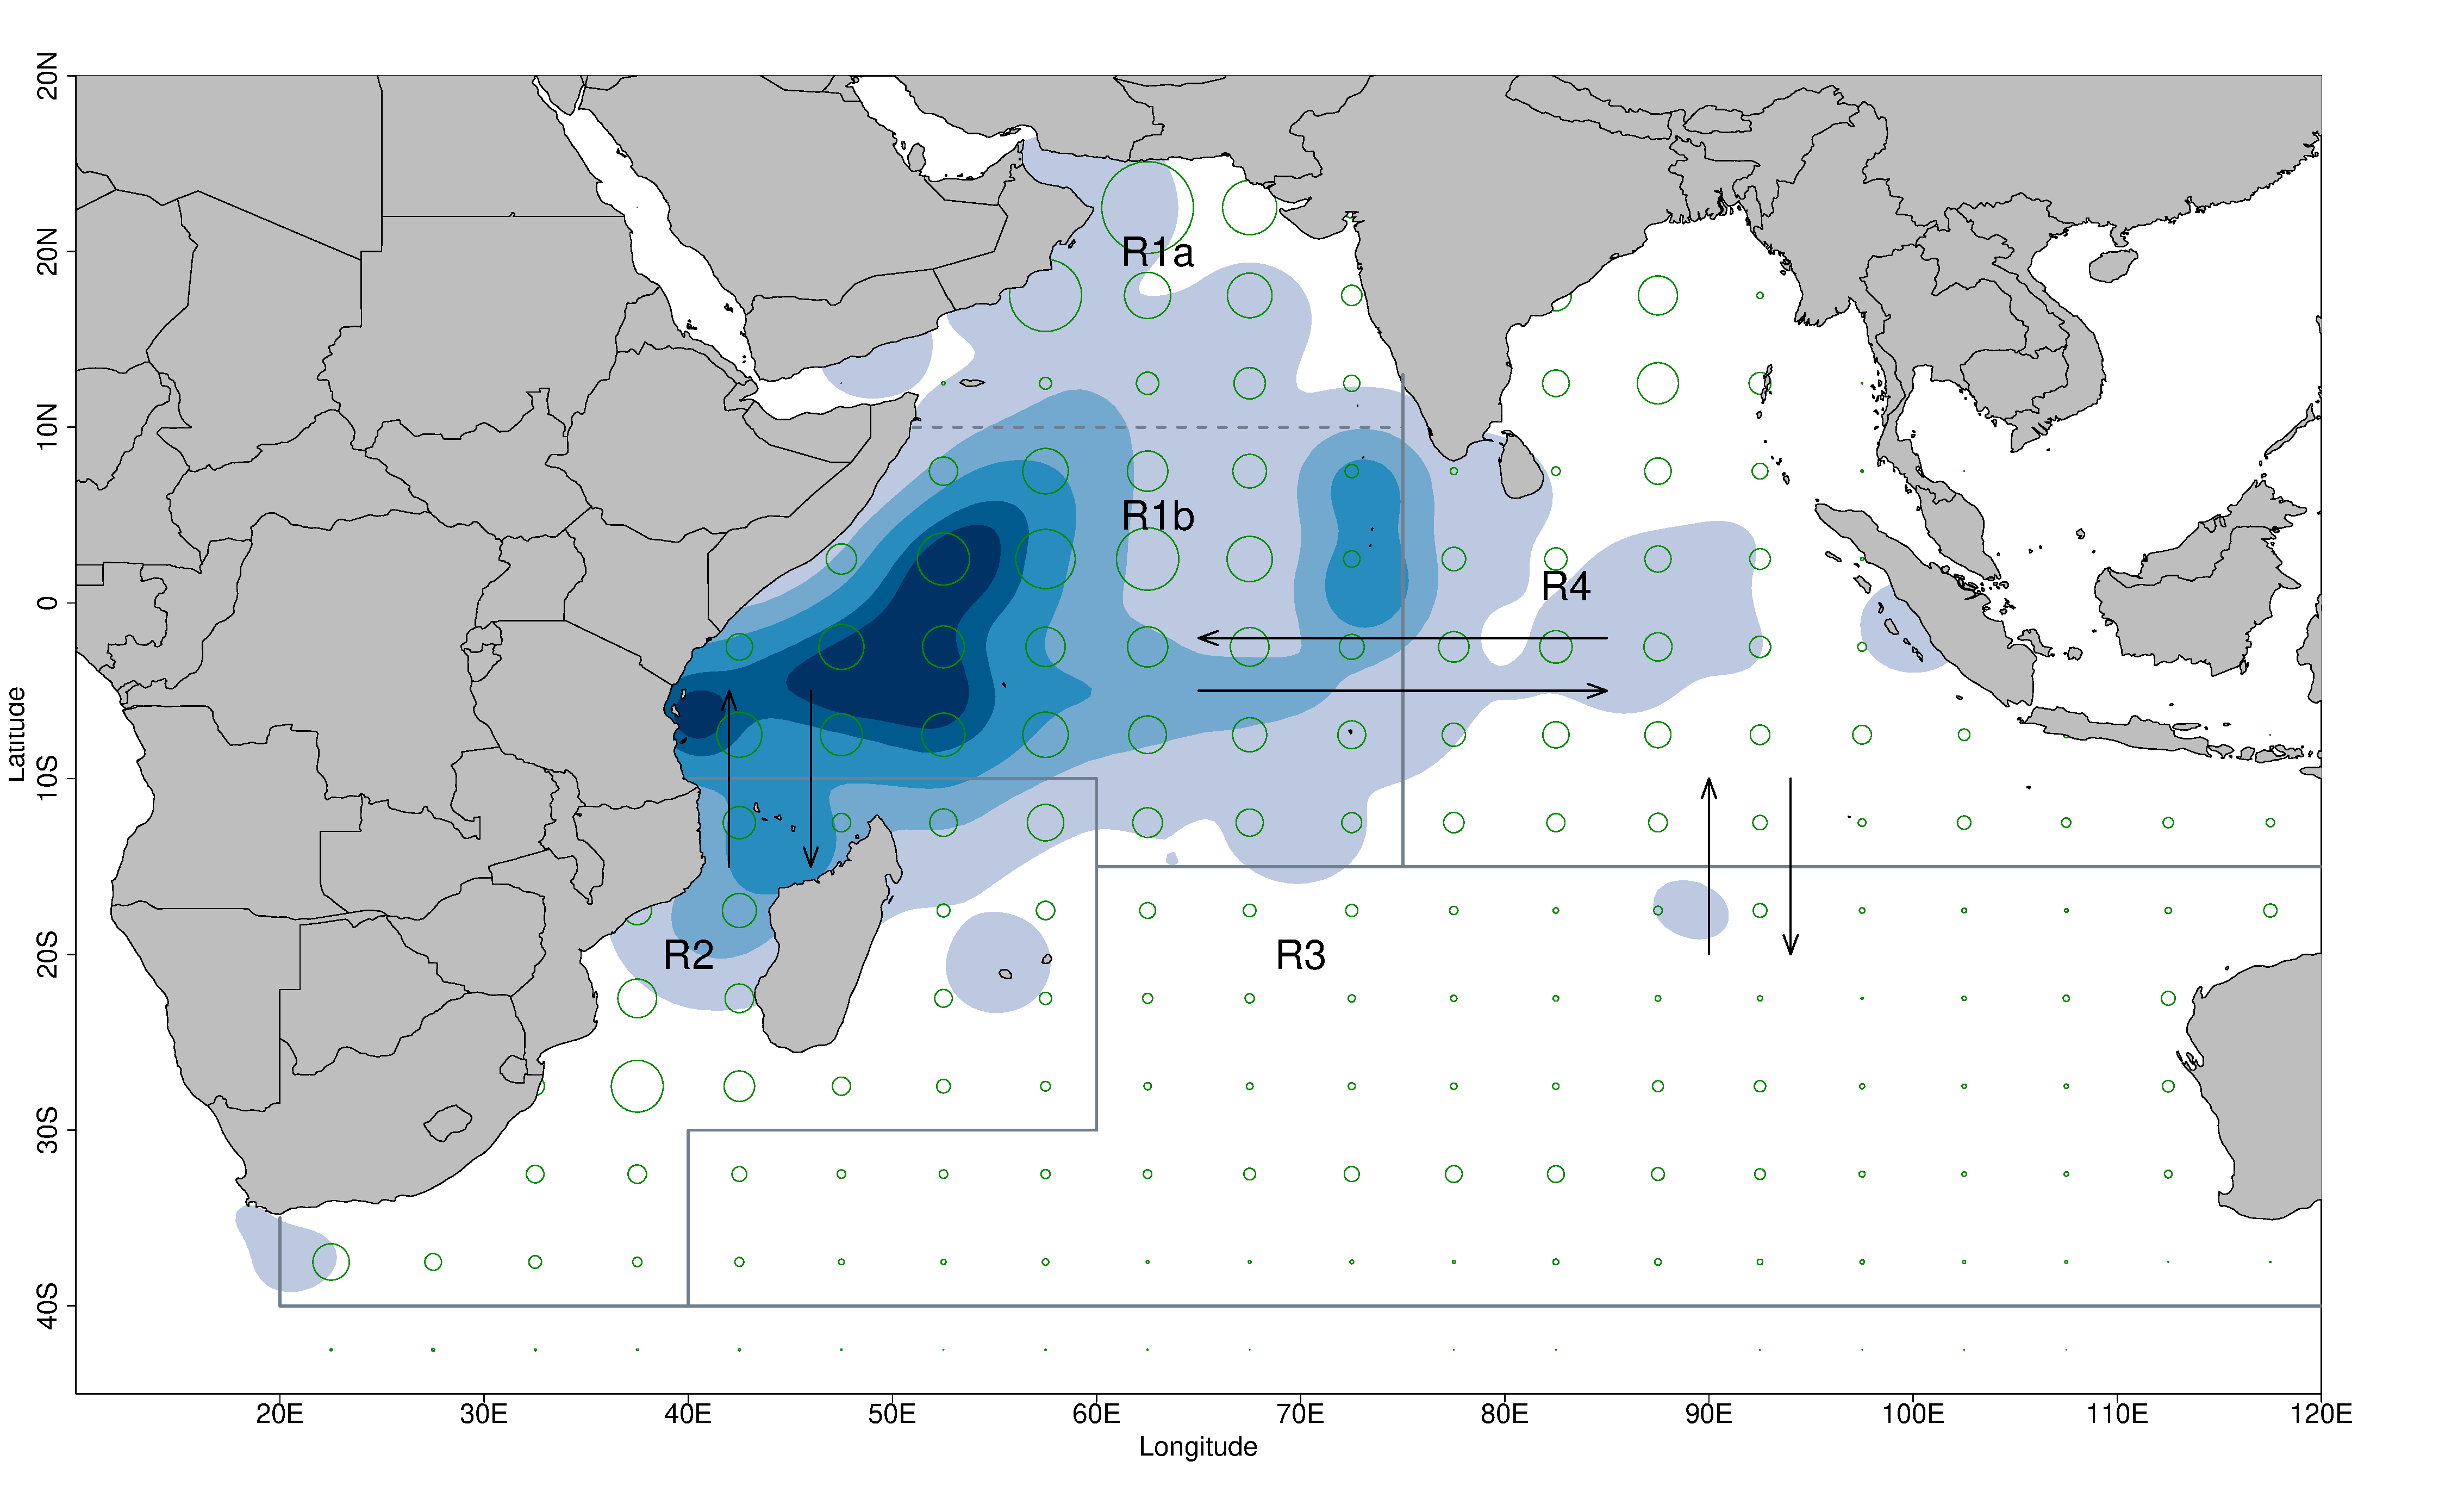
\includegraphics[width=6in]{fig1.eps}
\caption{Spatial stratification of the Indian Ocean for the four region assessment model (R1a and R1b were treated as a single model region R1 but were retained for the fleet definition). The black arrows represent the configuration of the movement parameterization.  Density contours represent of the dispersal of tag releases (red) and subsequent recaptures from Indian Ocean Regional tuna tagging programme. Green circles represent the distribution of catches from the longline fishery aggregated by 5 degree longitude and latitude for 1980 to 2017 (max. = 133 770 t).}
\label{fig:map}
\end{figure*}


\begin{figure}
\centering
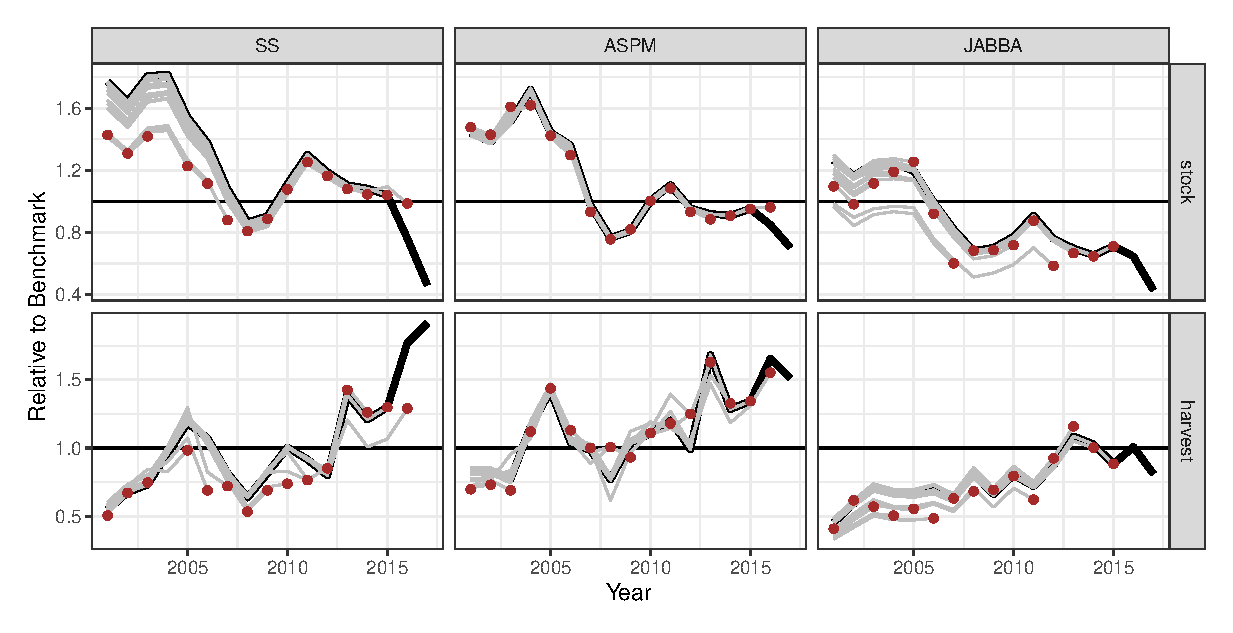
\includegraphics[width=6in]{fig2.eps}
\caption{Hindcasts for one-step for Stock Synthesis (SS),  Age-Structure Equilibrium Model (ASPM), and Bayesian state-space biomass dynamics model (JABBA).  The thick solid line represent the model estimates for relative stock quantities $stock$ and $harvest$ relative to $MSY$ benchmarks ($SSB$ and instantaneous fishing mortality for SS and ASPM and total biomass and harvest rate for JABBA). The points indicate the terminal years of the peels.}
\label{fig:retro}
\end{figure}


\begin{figure}
\centering
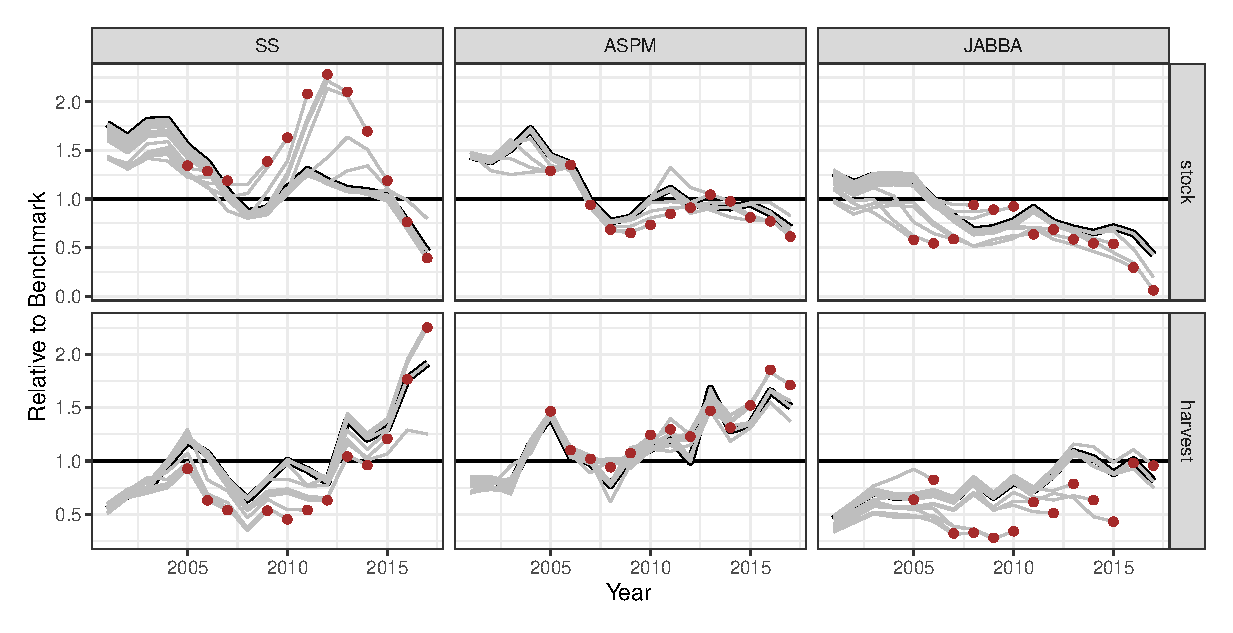
\includegraphics[width=6in]{fig3.eps}
\caption{Hindcasts for three-step for Stock Synthesis (SS),  Age-Structure Equilibrium Model (ASPM), and Bayesian state-space biomass dynamics model (JABBA).  The thick solid line represent the model estimates for relative stock quantities $stock$ and $harvest$ relative to $MSY$ benchmarks ($SSB$ and instantaneous fishing mortality for SS and ASPM and total biomass and harvest rate for JABBA). The points indicate the terminal years of the peels.}
\label{fig:retro3}
\end{figure}


\begin{figure*}[htbp]
\centering
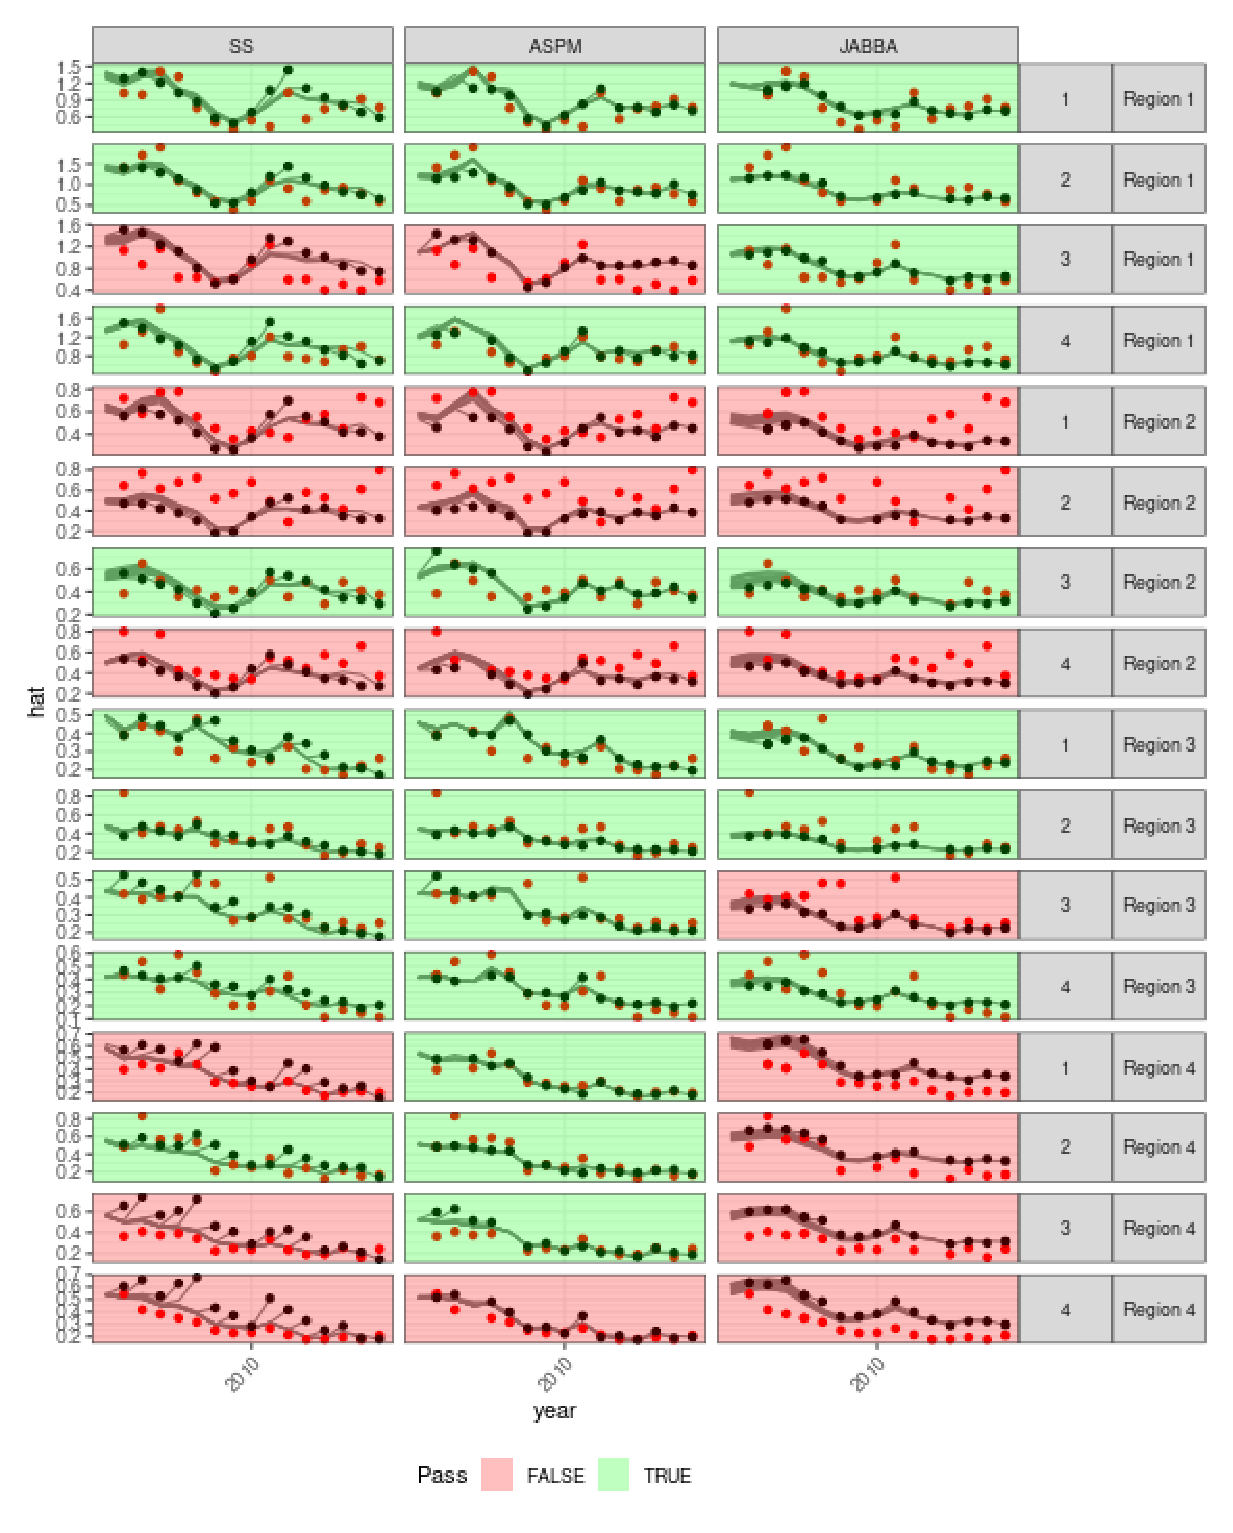
\includegraphics[width=6in]{fig4.eps}
\caption{Hindcasts with one year ahead projections for CPUE indices by region and quarter. Green backgrounds indicate that the CPUE index passes Mean Absolute Scaled Error (MASE < 1) criterion, or failed (red) otherwise. Red dots are the observed CPUE values and thin lines are the fits with terminal hincast year indicated by a solid point.}
\label{fig:hy}
\end{figure*}

\begin{figure*}[htbp]
\centering
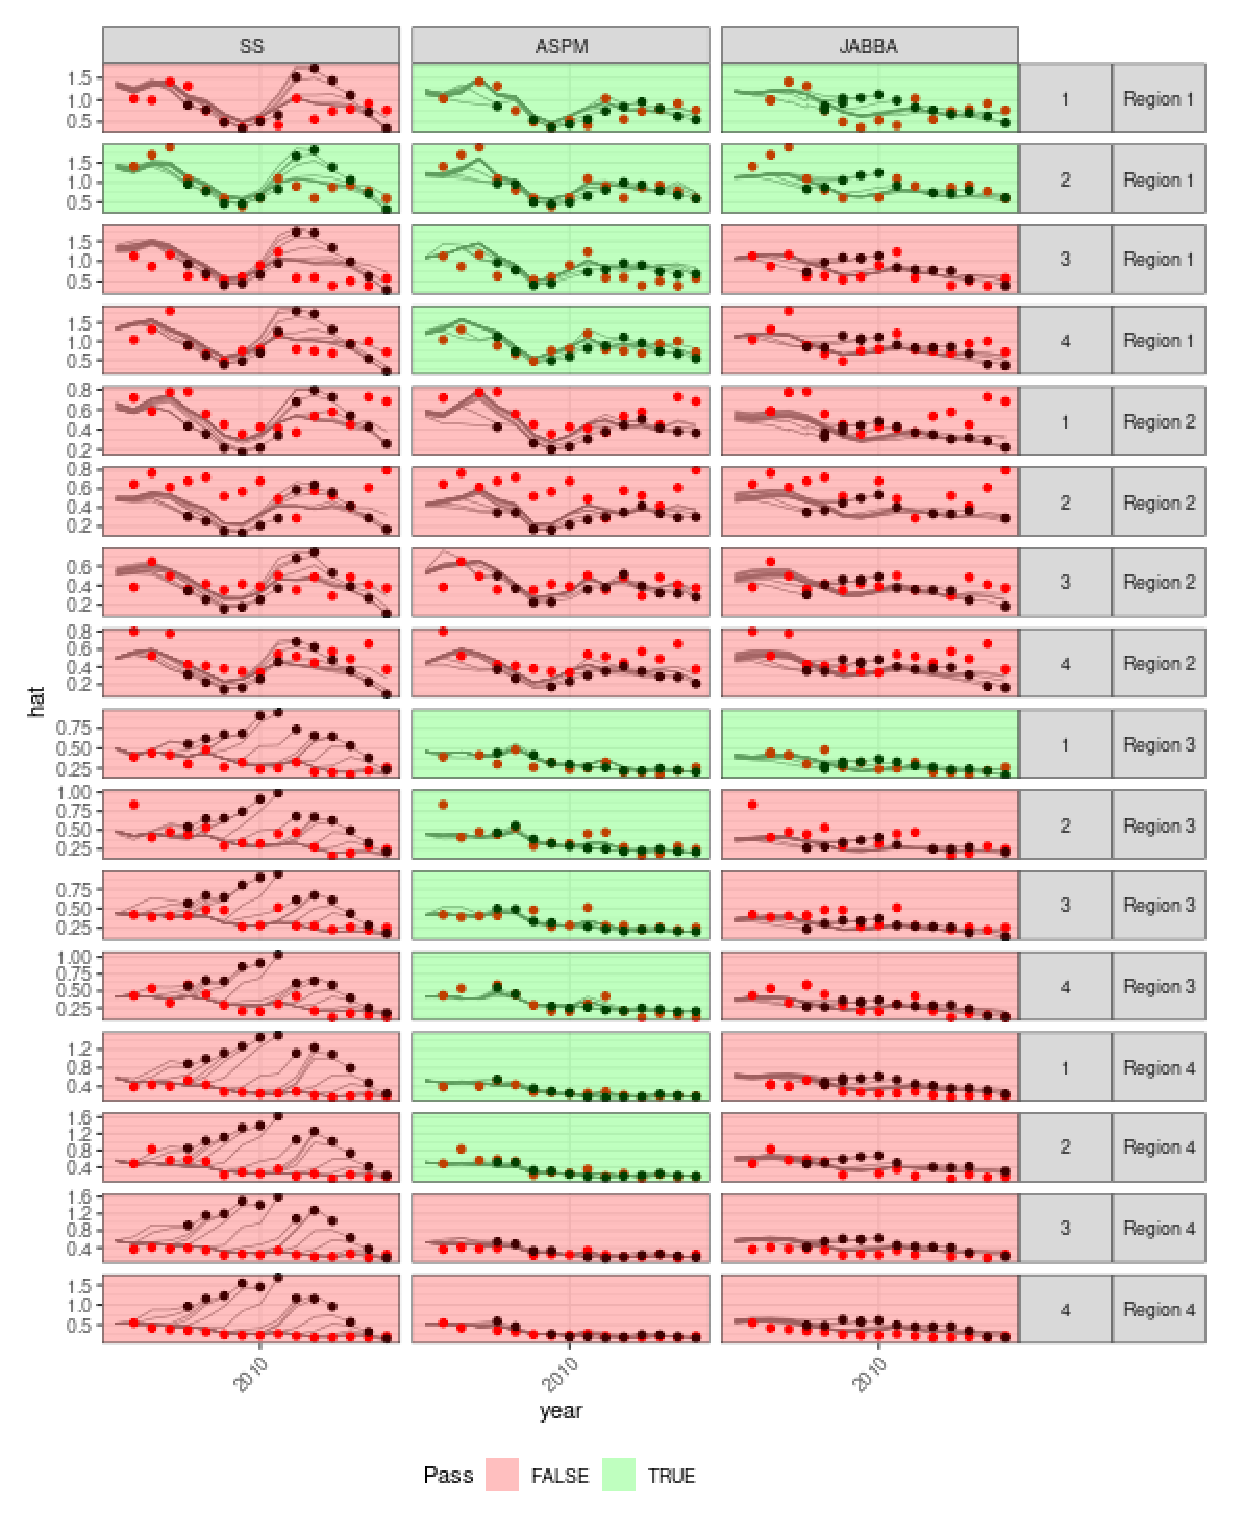
\includegraphics[width=6in]{fig5.eps}
\caption{Hindcasts for three year ahead projections for CPUE indices by region and quarter. Green backgrounds indicate that the CPUE index passes Mean Absolute Scaled Error (MASE < 1) criterion, or failed (red) otherwise. Red dots are the observed CPUE values and thin lines are the fits with terminal hincast year indicated by a solid point.}
\label{fig:hy3}
\end{figure*}

\begin{figure*}[htbp]
\centering
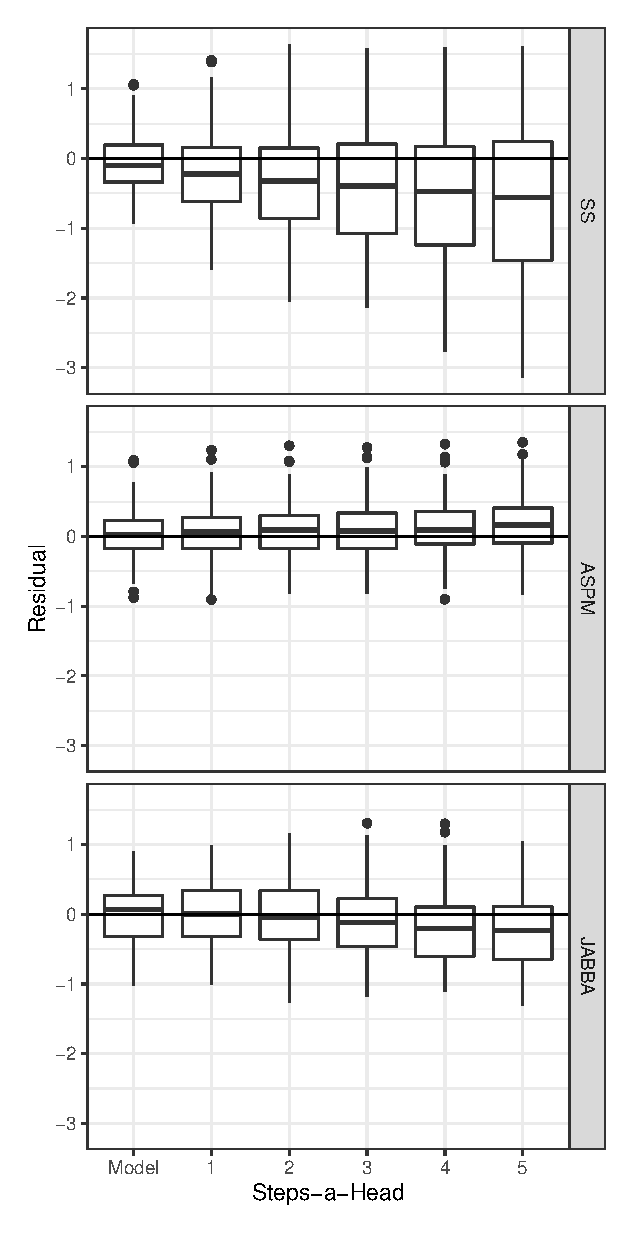
\includegraphics[width=4in]{fig6.eps}
\caption{Boxplots showing model residuals and prediction residuals for 1,2,3,4 and 5 year ahead projections, pooled for all CPUE indices across regions and quarters.}
\label{fig:residuals}
\end{figure*}

%\clearpage
%\newpage
%\subsection{Appendix}
%\label{metrics}

%\appendix* 
 %\subsection{Metrics}
%Indices of abundance are a key contributor to the overall likelihood when fitting stock assessment models to data. The Sum of Squared Errors (SSE) between observed and predicted indices in log-space is the measure of fitness. When comparing models, however, the SSE is problematic because complex models tend to have many parameters to allow flexibility when fitting, which may result in a low SSE due to overfitting. Therefore, information criteria, such as AIC, have been developed to aid in model selection. AIC is only a relative measure of the appropriateness of models, and additional diagnostic tests are required for model validation. This is of particular importance for stock assessment models where only a single historical data set exists, and the system can not be observed directly.

Therefore in stock assessment, a standard diagnostic is to evaluate retrospective bias as proposed by \cite{mohn1999retrospective}. As described in earlier sections, the retrospective analysis can be conducted by sequentially refitting the model to reduced data sets by removing some recent years' data to see if there are any systematic pattern within a model. The retrospective bias is then evaluated using the so-called Mohn's rho as 

\begin{equation}
\label{eqn:mohn0}
\rho_M = \disp \sum_{t=T-n}^{T-1} \frac{\hat{y}_{(1:t),t}-\hat{y}_{(1:T),t}}{\hat{y}_{(1:T),t}}, 
\end{equation}

where $\hat{y}$ denotes in general a value like estimated biomass, 1+population size, or predicted abundance index, and the value with suffix $\hat{y}_{(1:t^\prime),t}$ means such a value estimated at time $t$ of a full series from 1 to $T$ using a retrospective data window from 1 to $t^\prime (\leq T)$. In this paper, we will use a variant of the original $\rho$ as the mean (average) like 
\begin{equation}
\label{eqn:mohn}
\rho_{Mr} = \disp \frac{1}{n} \sum_{t=T-n}^{T-1} \frac{\hat{y}_{(1:t),t}-\hat{y}_{(1:T),t}}{\hat{y}_{(1:T),t}} 
\quad \mbox{[rho for retro-bias]}, 
\end{equation}
This metric is an average of relative differences at the final time of each window. Therefore it is a measure of relative retrospective `bias' (scale-free) in a statistical sense. The metric tends to be applied not on the log but the original scale because both the directions of positive and negative biases are regarded as being equivalent. 

To evaluate the absolute prediction error for the following can be used
\begin{equation}
\label{eqn:mohn3}
|\rho_p| = \disp \frac{1}{n-S+1} \sum_{t=T-n}^{T-S}
\frac{\left| \hat{y}_{(1:t),t+S}-\hat{y}_{(1:T),t+S} \right|}{\hat{y}_{(1:T),t+S}}. 
%\ \mbox{[rho for projection-absolute-error]}
\end{equation} 

Hindcasting, which is the primary focus in this paper is a form of retrospective cross-validation, and therefore an extension of retrospective analysis which projects several steps forward beyond the retrospective data window to quantify the prediction skill of a model. Theoretically, the projection period is to the end of the historical time period. However, in practice, the step size is one or several years ahead reflecting the requirements for robust management advice, and considering non-small process stochasticity in fishery population dynamics and non-ignorable extents of observation uncertainty. For evaluating prediction skill, we propose several metrics for model-dependent and model-free validations.

We  define `retro-period' and `hc-period' as `the period of shrunken data set for retrospective model fitting' and `future time period with a certain projection step (say $S \geq 1$) for hindcasting after retro-period''. And let $\hat{y}_{(1:t),t+S}$ be an projected value at time $t+S$ in an hc-period based on the conditioned model with data in a retro-period $(1,t)$. 

\vspace{0.2cm} \noindent
{\it Modified Mohn's rho for prediction bias and absolute error:}\\
\begin{equation}
\label{eqn:mohn2}
\rho_p = \disp \frac{1}{n-S+1} \sum_{t=T-n}^{T-S} 
\frac{\hat{y}_{(1:t),t+S}-\hat{y}_{(1:T),t+S}}{\hat{y}_{(1:T),t+S}} 
\ \mbox{[rho for projection-bias]}
\end{equation} 

This is a simple extension of Mohn's rho to evaluate the prediction skill of a model because all the values are produced under the model assumption. In this sense, it is a model-dependent consistency check of prediction skill. To evaluate the absolute prediction error for the following can be used
\begin{equation}
\label{eqn:mohn3}
|\rho_p| = \disp \frac{1}{(n-S+1)} \sum_{t=T-n}^{T-S}
\frac{\left| \hat{y}_{(1:t),t+S}-\hat{y}_{(1:T),t+S} \right|}{\hat{y}_{(1:T),t+S}}. 
\ \mbox{[rho for projection-absolute-error]}
\end{equation} 

There are problems with the use of relative error, since for reference model estimates which are low relative to the alternative model, i.e. $X_{ref} < X_{p}$, there is no upper limit, while for $X_{ref} > X_{p}$ the error cannot exceed 1.0. Therefore the chosen metric puts a heavier penalty on negative than on positive errors, i.e. historical underestimates. This means that when comparing models estimates, those that are low will be preferred. This problem can be overcome by using the logarithm of the ratio instead i.e. 
\begin{equation}
\label{eqn:re}
log\frac{X_{p}}{X_{ref}}
\end{equation}

which also leads to better statistical properties.


\vspace{0.2cm} 
The next three metrics are used for model-free validation, i.e. comparing predictions with observations. The error is defined as the difference between the predicted ($\hat{y}_{(1:t),t+S}$) and observed $y_{t+S}$) values, such as the model-based predicted CPUE using a retro-period data and observed CPUE used for model fitting. 

\vspace{0.2cm} \noindent
{\it Mean Absolute Percentage Error (MAPE) for projection:}
\begin{equation}
\label{eqn:mape}
MAPE = \disp \frac{1}{n-S+1} \sum_{t=T-n}^{T-S}
\frac{\left| \hat{y}_{(1:t),t+S}-y_{t+S} \right|}{y_{t+S}} \times 100 
\end{equation} 
A simple extension of the modified Mohn's rho for quantifying the relative difference between predictions and observations. This metric is also a scaled version of Mean Absolute Error (MAE). A problem with the MAE is that the relative size of the error is not always obvious. Sometimes it is hard to distinguish a big error from a small error. The MAPE can be calculated to allow forecasts of different series in different scales to be compared.

\vspace{0.2cm} \noindent
{\it Root Mean Squared Error (RMSE) for projection error:}\\
As an alternative measure of distance, the Mean Squared Error (MSE) is also commonly used in statistical literatures. To make comparison easier, the following squared root variant of MSE can be used: 
\begin{equation}
\label{eqn:rmse}
RMSE = \disp \sqrt{ \frac{1}{n-S+1} \sum_{t=T-n}^{T-S} 
\left( \hat{y}_{(1:t),t+S}-y_{t+S} \right)^2 }
\end{equation} 

In comparison to $\rho_p$ and MAPE, RMSE is not scale-invariant and can be influenced by large discrepancies in a single data point. A useful feature, however, that the squared RMSE can, in general, be expressed,  for a notational simplicity if we set $S$ at 1, as

\begin{equation}
\label{eqn:rmse2}
\begin{array}{lcl}
\vspace{0.1cm}
{RMSE}^2 &=& \disp \frac{1}{n} \sum_{t=T-n}^{T-1} \left( \hat{y}_{(1:t),t+1}-y_{t+1} \right)^2 \\
\vspace{0.1cm}
&=& \disp \frac{1}{n} \sum_{t=T-n}^{T-1} \left( \hat{y}_{(1:t),t+1}-y_{t+1} - \bar{E} \right)^2 + \bar{E}^2 \\
&=& \disp E^{\prime 2} + \bar{E}^2
\end{array}
\end{equation}
where 
\begin{equation}
\begin{array}{lcl}
\vspace{0.1cm}
\bar{E} &=& \disp \frac{1}{n} \sum_{t=T-n}^{T-1} \left( \hat{y}_{(1:t),t+1}-y_{t+1} \right), \\
\vspace{0.1cm}
E^{\prime 2} &=& \disp \frac{1}{n} \sum_{t=T-n}^{T-1} \left( \hat{y}_{(1:t),t+1}-y_{t+1} - \bar{E} \right)^2.
\end{array}
\end{equation}
The centred mean squared error, $E^{\prime 2}$ can be also expressed as 
\begin{equation}
E^{\prime 2} = \sigma_o^2 + \sigma_f^2 - 2\sigma_o \sigma_f Cor,
\end{equation}
where $\sigma_o$ and $\sigma_f$ are respectively the standard deviation of observation $y_t$ and prediction, and $Cor$ is the correlation between them. This means that $E^\prime$, $\rho$ and $\sigma_f$ can be summarised simultaneously \parencite{taylor2001summarizing}. Taylor diagrams provide a concise statistical summary of how well patterns match each other and are therefore useful for evaluating multiple aspects or in gauging the relative skill of different models \parencite{griggs2002climate}. It should be remarked that RMSE can be extended for a percentage measure as MAPE, but for the reason stated below, we use RMSE as defined above 

\vspace{0.2cm} \noindent
{\it Mean absolute scaled error (MASE) for projection:}\\ 
A more robust and easier to interpret statistic for evaluating prediction skill is the MASE \parencite{hyndman2006another}. MASE evaluates a model's prediction skill relative to a na\" {i}ve baseline prediction, based on previous observation. A prediction is said to have skill if it improves the model forecast compared to the baseline. A widely used baseline forecast for time series is the persistence algorithm that takes the value at the previous time step to predict the expected outcome at the next time step as a na\ "{i}ve in-sample prediction, i.e. tomorrow weather will be the same as today. The original definition of MASE for 1-step ahead prediction is 
\begin{equation}
\label{eqn:mase}
{MASE=\frac{\disp \frac{1}{n} \sum_{t=T-n}^{T-1} \left| \hat{y}_{(1:t),t+1}-y_{t+1} \right|}
{\disp \frac{1}{n-1} \sum_{t=T-n+1}^{T-1} \left|y_{t+1}-y_{t}\right|}}, 
\end{equation}
and this can be extended as \toshi{actually not very much straightforward but seems as below}
\begin{equation}
MASE=
\frac{\disp \frac{1}{n-S+1} \sum_{t=T-n}^{T-S}  \left| \hat{y}_{(1:t),t+S}-y_{t+S} \right|}
{\disp \frac{1}{n-S} \sum_{t=T-n+1}^{T-S} \left|y_{t+S}-y_{t}\right|}. 
\end{equation} 
The MASE has the desirable properties of scale invariance, predictable behaviour, symmetry, interpretability and asymptotic normality. Compared to MAPE, which relies on the division by observations for scaling, MASE does not necessarily skew its distribution even when the observed values are close to zero. MASE is also easier to interpret as a score of 0.5 indicates that the model forecasts are twice as accurate as a na\''{i}ve baseline prediction; the model thus has prediction skill.
\vspace{0.2cm} 
The best statistical measure to use depends on the objectives of the analysis and using more than one measure can be helpful in providing insight into the nature of observation and process error structures. Here for the evaluation of models, we will use the following metrics: 

\begin{itemize}
\item Original Mohn's rho ($\rho$) for checking the retrospective bias \\
\vspace{-0.3cm}
\item Modified Mohn's rho for prediction \toshi{bias and absolute error, which? both might be meaningful though but it becomes noisy...} as checking model-based self-consistency check \\
\vspace{-0.3cm}
\item MASE and RMSE for model-free validation with different angles. 
\end{itemize}


\end{document}

We wish to submit this paper for the special issue in commemoration of Sidney Holt, however, if not thought appropriate we would like it to be considered for a regular issue. 

The reason for submission to the special issue is because of discussions at the World Fisheries Conference (Cadrin and Dickey-Collas, 2014) where Sidney argued that the definition of stock assessment was ``The description of the characteristics of a 'stock' so that its biological reaction to being exploited can be rationally predicted and the predictions tested"  There was a lot of discussion but no resolution.

Our support for Sidney's reasoning was because this explicitly recognises that an aim of stock assessment is to provide the basis for the long-term sustainable management of fisheries, which Sidney's work laid the foundations for. Stock assessment, therefore, requires making and validating probabilistic estimates of stock status and forecasts of the consequences of management actions". This prompted a lot of debate but no clear conclusion, and we have written this paper in memory of Sidney.

Cadrin, Steven X and Mark Dickey-Collas (2014). “Stock assessment methods for sustainable fisheries”. In:ICES Journal of Marine Science72.1, pp. 1–6

